%! Date = 18/07/2022

\documentclass[a4paper,11pt,draft=false,bibliography=totoc]{scrartcl} % scrartcl scrreprt scrbook

\usepackage{ebgaramond} % gillius ebgaramond
\usepackage{amsmath}
\usepackage[ngerman]{babel}
\usepackage{relsize}
\usepackage{caption}
\usepackage{tabularx}
\usepackage[newfloat=true]{minted}
\usepackage{pdfpages}
\usepackage[utf8]{inputenc}
\usepackage[automake]{glossaries-extra}
\usepackage[onehalfspacing]{setspace}
\usepackage{graphicx}
\usepackage{csquotes} % dependency of biblatex
\usepackage{biblatex}
\usepackage{xcolor}
\usepackage{newfloat}
\usepackage[section]{placeins} % keep figures near declaration inside Anhang

\bibliography{refs}

\setlength{\parindent}{0pt} % disable weird indentation after \begin...\end sections for now
\graphicspath{ {./images/} }

\makeglossaries

\newglossaryentry{Textpassage}
{
    name=Textpassage,
    description={Ein Stück Text aus einer Textdatei. Dabei
            wird sich meist auf eine in der Konfigurationsdatei spezifizierte
            Zieldatei des Programms bezogen.}
}

\newglossaryentry{Zielmuster}
{
    name=Zielmuster,
    description={Ein Element innerhalb der Konfigurationsdatei. Es bezeichnet ein
            Stück Text das einen speziellen \gls{Platzhalter}, den Text \mintinline{bash}{{{value}}},
            enhält. Es wird vom Programm dazu genutzt den genauen Ort der Ziel-\gls{Textpassage}
            innerhalb der Zieldatei zu identifizieren. Das Zielmuster sollte}
}

\newglossaryentry{Platzhalter}
{
    name=Platzhalter,
    description={Ein vordefinierter Text: das englische Wort \mintinline{bash}{value}
            umgeben von doppelten geschweiften Klammern:
            \mintinline{bash}{{{value}}} Das Format des Platzhalters ist an die
            die Template-Engine Template-Engine Jinja2 \cite{jinja2} angelehnt.
            Er ist Teil des \gls{Zielmuster}s das zusätzlich Text vor und nach
            der Ziel-\gls{Textpassage} enthält. Er markiert den Ort der Ziel-\gls{Textpassage}
            relativ zum \gls{Zielmuster} innerhalb der Zieldatei.}
}

\newglossaryentry{Property-Based-Testing}
{
    name=Property-Based-Testing,
    description={Property-Based-Testing bezeichnet eine spezielle Strategie Softwaretests
            zu formulieren. Statt einer Reihe explizit ausformulierter Tests wird eine Regel
            formuliert, welcher das zu testende Programm für automatisch generierte Eingabewerte
            genügen muss.}
}

\glsaddall

\author{Adrian Schurz}
\title{Terminal-Config-Manager\\
	Informatik für Anwendungsentwicklung\\
	CHECK24 Tech Hub und Services GmbH\\
	}

\begin{document}

\definecolor{codebg}{rgb}{0.95,0.95,0.95}

\maketitle
\pagenumbering{gobble}
\newpage

\section{Projektantrag}
\begin{center}
	Diese Seite wird später entfernt.
\end{center}
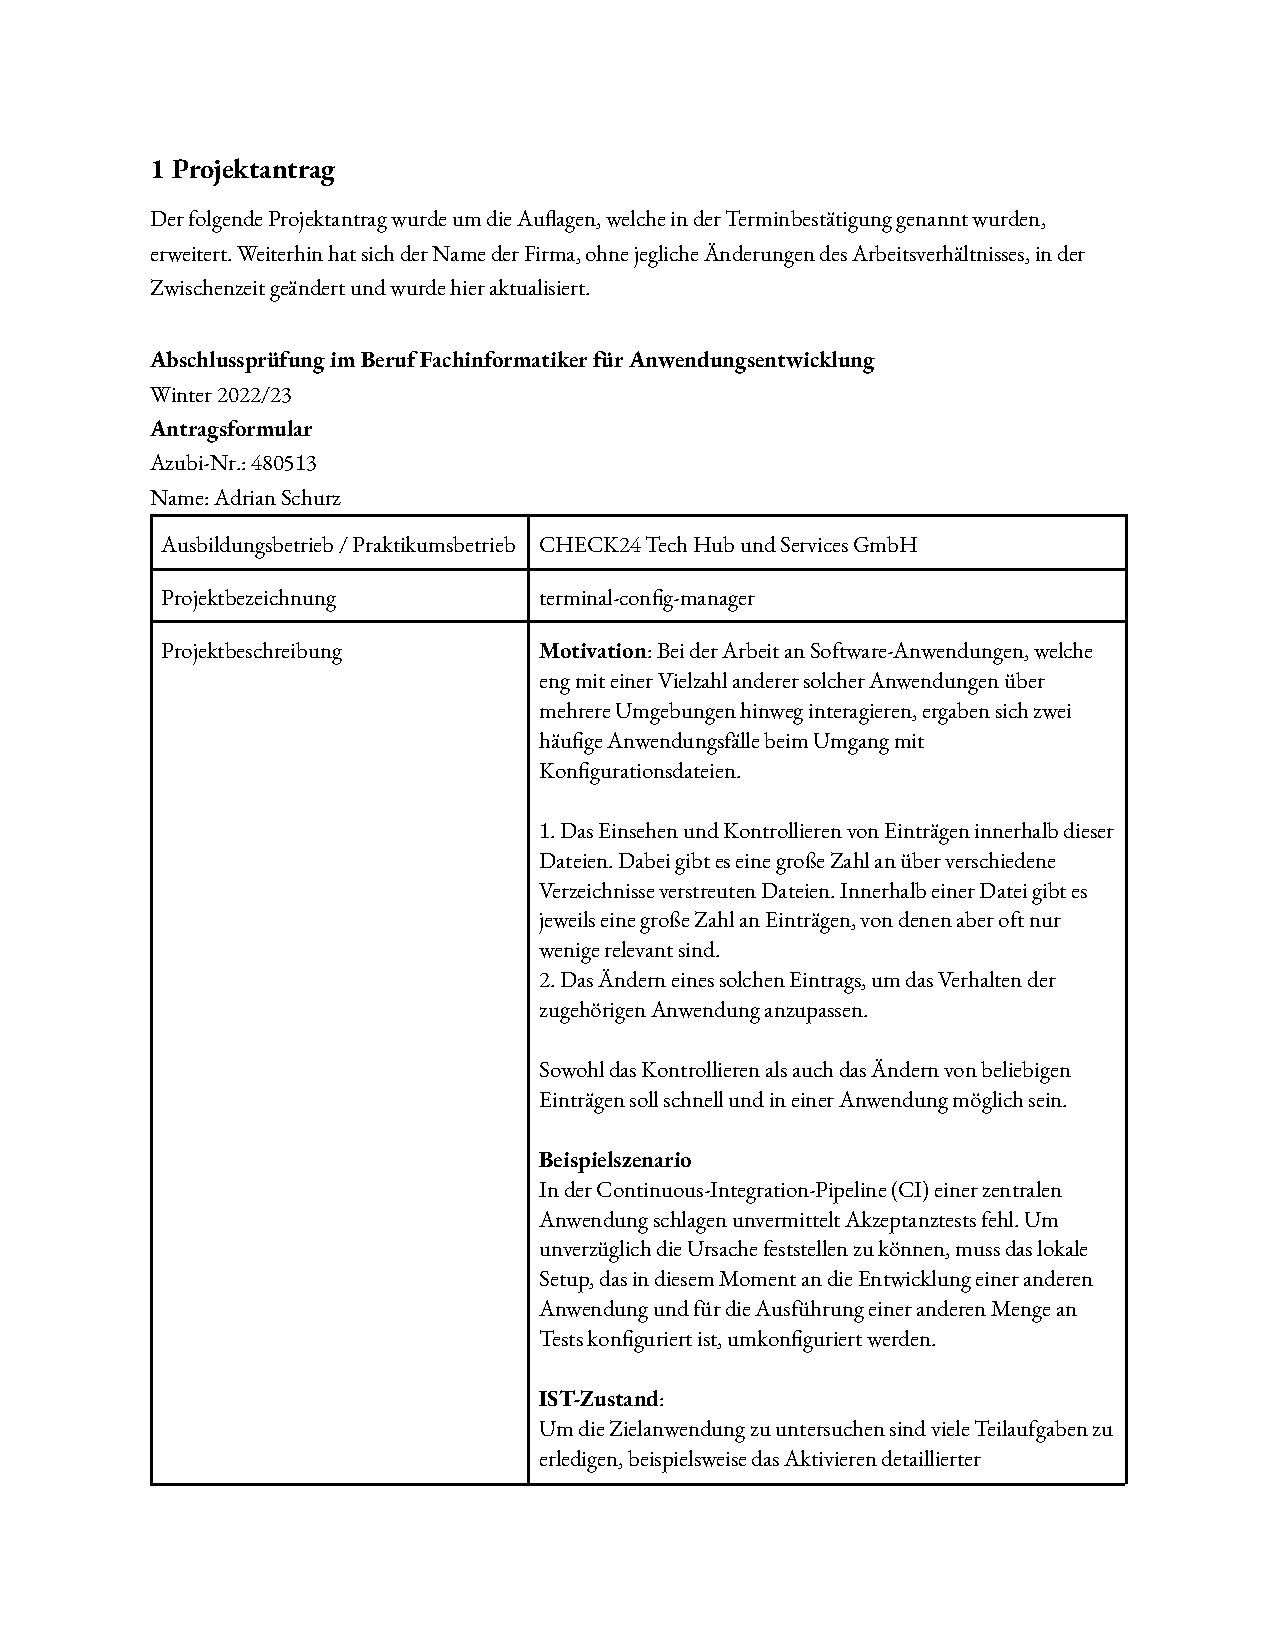
\includepdf[pages={-}]{../projektantrag/projektantrag_final.pdf}

\section{Nachweisblatt} \label{Nachweisblatt}
\paragraph{}

\newpage
\tableofcontents
\newpage

\pagenumbering{arabic}

\section{Textteil - vorläufiger Titel} \label{Textteil}

\subsection{Problemstellung}
\paragraph{}
Der Bedarf für die im Rahmen dieser Projektarbeit erstellte Softwarelösung ergab
sich bei der Arbeit an Software-Anwendungen, welche eng mit einer Vielzahl
anderer solcher Anwendungen über mehrere Umgebungen hinweg interagieren.

\paragraph{}
Der Großteil dieser Anwendungen besitzt weitläufige Konfigurationsmöglichkeiten
welche ihren Betrieb in verschiedensten Szenarien steuern. Beispiele für
Konfigurationsmöglichkeiten und deren Ausprägungen sind:

\begin{itemize}
    \item Das Loggingverhalten der Anwendung
          \begin{itemize}
              \item Logging gegen die Logverarbeitungssoftware der Produktionsumgebung
              \item Logging gegen eine lokale Instanz der Logverarbeitungssoftware
              \item Logging auf das Dateisystem
              \item Logging mit verschiedenen Logleveln
          \end{itemize}
    \item Die Zieldatenbank der Anwendung \begin{itemize}
              \item Datenbank der Produktionsumgebung
              \item Datenbank der Testumgebung
              \item lokale Datenbank
          \end{itemize}
    \item Die Ausführung von Softwaretests \begin{itemize}
              \item Ausführen von ausschließlich Unittests
              \item Ausführen von Akzeptanztests
              \item Ausführen der Gesamtheit der Tests
              \item Anpassung der Ziel-IP einer weiteren, für die Testausführung
                    notwendigen Anwendung
          \end{itemize}
    \item uvm.
\end{itemize}

\paragraph{}
Der Kontext der Arbeit an der Software wechselt regelmäßig zwischen Entwicklung und
dem Suchen bzw. Nachvollziehen von potentiellen Softwarefehlern, welche im Produktions-
oder Testbetrieb auftreten. Um dabei das beobachtete Verhalten der Anwendung korrekt
zu interpretieren sind u.a. zwei Arbeitsschritte häufig zu erledigen:

\begin{itemize}
    \item \textbf{Prüfen} der aktuellen Konfiguration
    \item \textbf{Anpassen} der aktuellen Konfiguration
\end{itemize}

Die Anzahl der an jedem Einzelfall beteiligten Anwendungen und die Anzahl der
Konfigurationsdateien pro Anwendungen führen dazu, dass jeweils viele verschiedene
und weit über das Dateisystem verstreute Dateien relevant sind. Pro Datei und
Einzelfall sind folgende Arbeitsschritte zu erledigen:

\begin{itemize}
    \item Starten der zur Anwendung gehörigen IDE
    \item Ermitteln der Konfigurationsdatei
    \item Navigation im Verzeichnisbaum
    \item Öffnen der Datei
    \item Finden des relevanten Eintrags in einer mitunter sehr langen Textdatei
    \item Ermitteln der möglichen Zielwerte
    \item Ändern des Eintrags
    \item Speichern der Datei
\end{itemize}

Diese Einzelschritte, mulipliziert mit der Anzahl an Dateien, stellt eine
Menge an repetitiven Handlungen dar die, wenn sie erleichtert würden, Zeit und
Konzentrationsvermögen einsparen können.

\paragraph{Ziel}
dieser Projektarbeit ist es ein Programm zu entwerfen und zu implementieren
welches die beschriebenen Arbeitsschritte bestmöglich vereinfacht und beschleunigt.


\section{Technologie}
\subsection{Kriterien}
\paragraph{}
Für dieses Projekt bieten sich grundsätzlich alle gängigen Programmiersprachen
an. Während der Umsetzung soll ausgewählten Aspekten der Softwareentwicklung
gesonderte Aufmerksamkeit zukommen.

\paragraph{Korrektheit und Laufzeitstabilität} Es soll auf technischem Weg zum
Einen sichergestellt werden, dass sich das Programm zu jedem Zeitpunkt erwartungsgemäß
und korrekt verhält und zum Anderen, dass Fehlerzustände zur Laufzeit so weit
wie möglich ausgeschlossen werden.

\paragraph{}
Als hauptsächliche Wege dies zu erreichen werden folgende Ansätze gewählt:

\begin{itemize}
    \item Wahl einer Programmiersprache mit strenger Typisierung
    \item Wahl einer kompilierten Programmiersprache mit vergleichsweise starken
          Garantien zum Laufzeitverhalten
    \item Einbeziehung von \gls{Property-Based-Testing} \cite{property-based-testing} in das Konzept der Softwaretests
\end{itemize}

\paragraph{Ausführliche, vom Quellcode abgeleitete Moduldokumentation}
Neben der Projektdokumentation soll eine Dokumentation der einzelnen
Softwaremodule entstehen. Um dem Problem zu begegnen, dass Dokumentation und
Quellcode im Laufe der Entwicklung auseinanderlaufen soll die Moduldokumentation
direkt aus den Quellcodekommentaren generierbar sein.

\subsection{Auswahl}
Als Programmiersprache und Build-System wurden auf Basis der obengenannten Ziele
Haskell \cite{haskell} und Stack \cite{stack} gewählt.

\paragraph{}
Stack bietet neben seiner Hauptaufgabe die Software-Abhängigkeiten des Projekts
zu verwalten und den Buildvorgang zu steuern die Möglichkeit Moduldokumentation
im HTML-Format anhand der Quellcodestrukur und der Quellcodekommentare generieren
während Haskell eine typsichere, kompilierte Programmiersprache mit Unterstützung
für \gls{Property-Based-Testing} darstellt.

\subsection{Projektorganisation}
% include generated documentation

\subsection{Design}
% include domain driven design

\section{Ergebnisdiskussion}

\subsection{Funktionalität}
Die Hauptfunkionalität des Programms wurde erfolgreich umgesetzt und es wird von
mir selbst bereits genutzt. Das Programm arbeitet seither wie erwartet,
ist konfigurierbar und informiert mit lesbaren Nachrichten im Falle eines Fehlers.
Ein weiteres Feature wäre jedoch wünschenswert, die Fähigkeit des Programms mit
schreibgeschützten Zieldateien umgehen zu können und in diesem Fall eine
sudo-Passwortabfrage auszulösen. Letzteres ist nicht Teil der
usprünglichen Anforderungen und wird daher erst zukünftig umgesetzt.

\subsection{Domain Driven Design}
Das Ziel die Abhängigkeiten der einzelnene Softwaremodule untereinander einem
mit dem Domain-Driven-Design kompatiblen Schema folgend zu organisieren ist mit
einer Ausnahme geglückt. Im Anhang, Abb. \ref{domain-driven-design-layers}, sind Module
der Applikationsebene abhängig von Modulen des User-Interface. Das verwendete
\gls{GUI}-Framework, Brick, führt durch sein Interface allerdings zu einem Muster bei
dem diese Abhängigkeit umgekehrt ist. Letzteres wird deutlich beim Vergleich des Schemas mit den
tatsächlichen Modulabhängigkeiten (siehe Abb. \ref{module-dependency-graph} im Anhang).
Dieser Umstand stellt für den Moment eine vernachlässigbare Designschwäche dar die ohne weitere
Konquenz ist. Aus diesem Grund erhielt die Aufgabe dies zu beheben eine niedrige
Priorität und steht vorerst noch aus. Alle sonstigen Module halten das angestrebte
Schema ein.

\subsection{Moduldokumentation}
Das Ziel die Moduldokumentation ständig, während des Buildprozesses, aktuell zu
halten ist teilweise geglückt. Im Projektverzeichnis liegt die ausführliche Moduldokumentation
einschließlich jener der eingebundenen Softwarebibliotheken im HTML-Format vor.
Auszüge davon sind in den Abbildungen \ref{module-doc-index} und \ref{module-doc-state} dargestellt.
Allerdings gibt es seit wenigen Tagen bei neueren Versionen des Buildsystems Stack \cite{stack}
und des Generierungstools Haddock \cite{haddock} eine Inkompatibilität. Bis diese
in diesen Projekten behoben und veröffentlicht ist, ist die in diesem Projekt hinterlegte
Moduldokumentation nicht aktuell. Es ist zu erwarten, dass dieses Problem in naher
Zukunft seitens der Entwickler der beiden Tools behoben wird.

\subsection{Testabdeckung}
Die Abdeckung der Funktionalität des Programms auf Unittest-Ebene ist, besonders
dank der Verwendung von \gls{Property-Based-Testing} \cite{property-based-testing}
zufriedenstellend.

\paragraph{}
Eines der angestrebten Ziele war jedoch neben ausführlichen Unittests ebenso ausführliche
Akzeptanztests bereitzustellen. Dies ist trotz erheblichem Aufwand gescheitert.
Das Programm ist eine Konsolenanwendung, welche auf Tasteneingaben reagiert. Das
bedeutet, dass automatisierte Tests in einer kontrollierten Umgebung Terminal-Emulatoren
starten und ihnen Tasteneingaben simulieren müssen um das Programm zu testen. Je nach
der verwendeten grafischen Benutzeroberfläche des Betriebssystems unterscheiden sich
die Ansätze dies zu erreichen jedoch stark. Es existieren mehr oder weniger gut
gepflegte Open-Source-Softwaretools für die Teilaufgabe der Eingabeemulation. Verschiedene
Kombinationen dieser Tools (xdotool \cite{xdotool} vs ydotool \cite{ydotool}) wurden
mit verschiedenen Displayservern (xorg \cite{xorg} vs. wayland \cite{wayland}),
Betriebssystemen (Ubuntu \cite{ubuntu} vs Arch Linux \cite{arch}), und
Virtualisierungslösungen (virtualbox \cite{virtualbox} vs docker \cite{docker})
evaluiert. Keine der Varianten führte zum Erfolg.

\subsection{Bekannte Fehler}
Es sind zwei Bugs in Software-Abhängigkeiten des verwendeten \gls{GUI}-Frameworks
bekannt, welche mit geringer Häufigkeit das \gls{Rendering} bzw. den Start des Programms
beeinträchtigen. Diese Bugs sind dokumentiert (siehe \cite{bug-vty-startup-crash} und
\cite{bug-vty-terminal-capabilities}). Einer dieser Fehler führt dazu, dass der
aktuelle Wert eines Eintrags weiß statt blau gerendert wird und ist schwer
reproduzierbar (1x ca. pro 50-100 Programmstarts). Der andere Fehler führt zu
einem Crash des Programms beim Start (1x ca. pro 30-50 Programmstarts).



\section{Anhang} \label{Anhang}

\begin{figure}[ht]
    \caption{Generierte Moduldokumentation, Hauptseite}
    \label{module-doc-index}
    \fbox{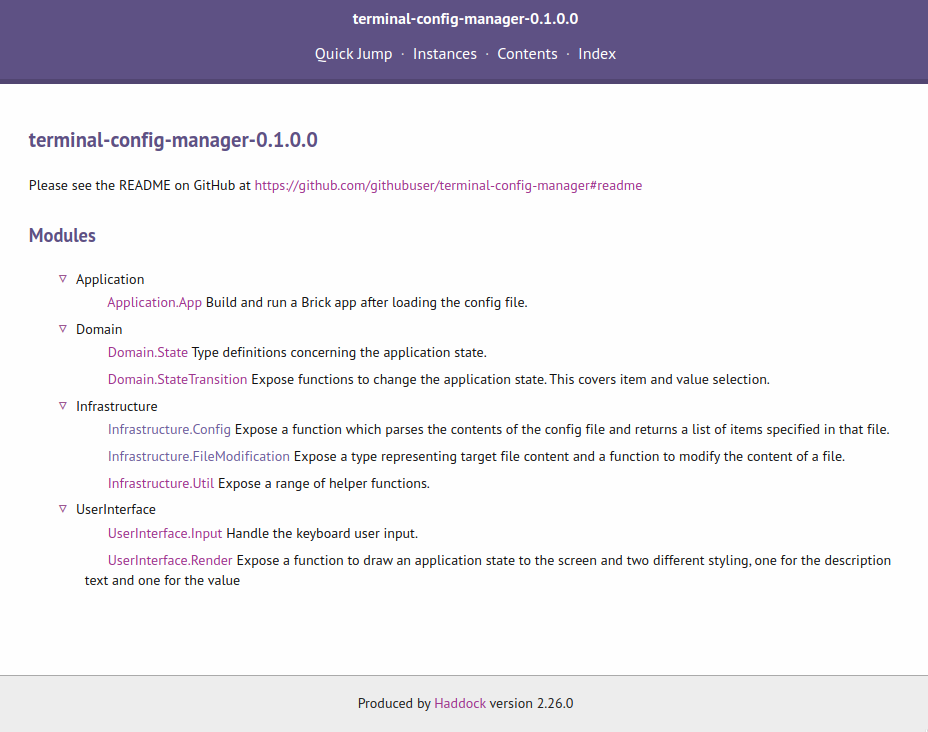
\includegraphics[scale=0.5]{module-documentation-index.png}}
\end{figure}

\begin{figure}[ht]
    \caption{Generierte Moduldokumentation, Domain.State}
    \label{module-doc-state}
    \fbox{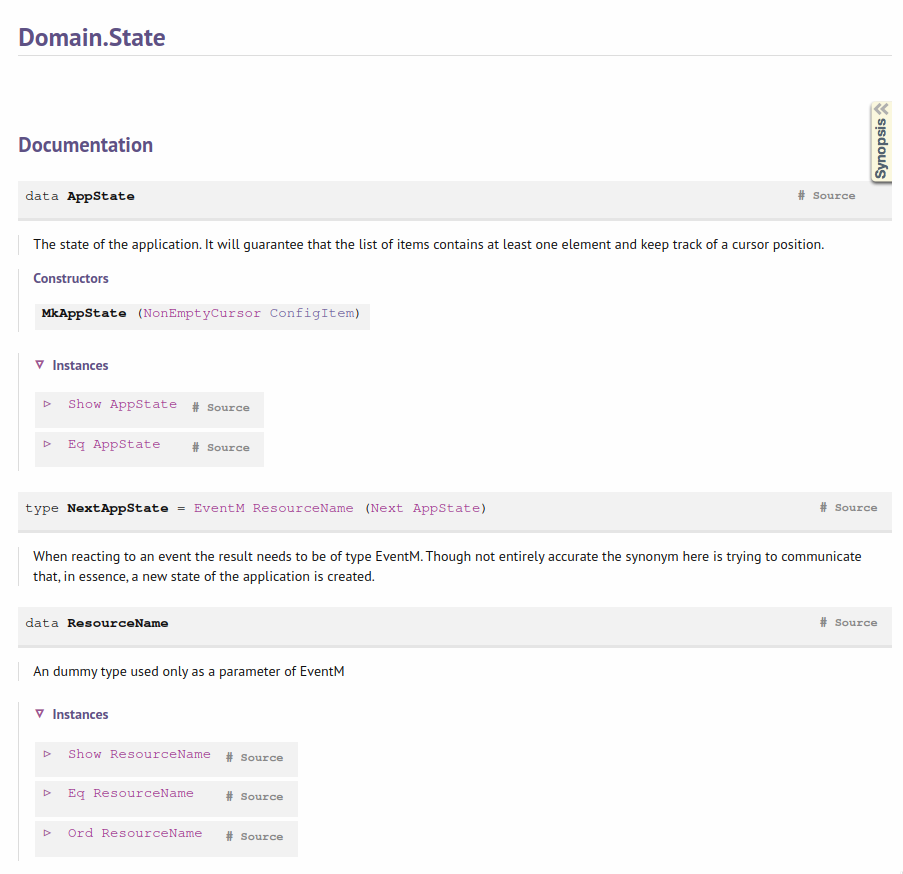
\includegraphics[scale=0.5]{module-documentation-state.png}}
\end{figure}

\begin{figure}[ht]
    \caption{Beispielschema für Modulabhängigkeiten beim Domain-Driven-Design \cite{domain-driven-design}}
    \label{domain-driven-design-layers}
    \centering\fbox{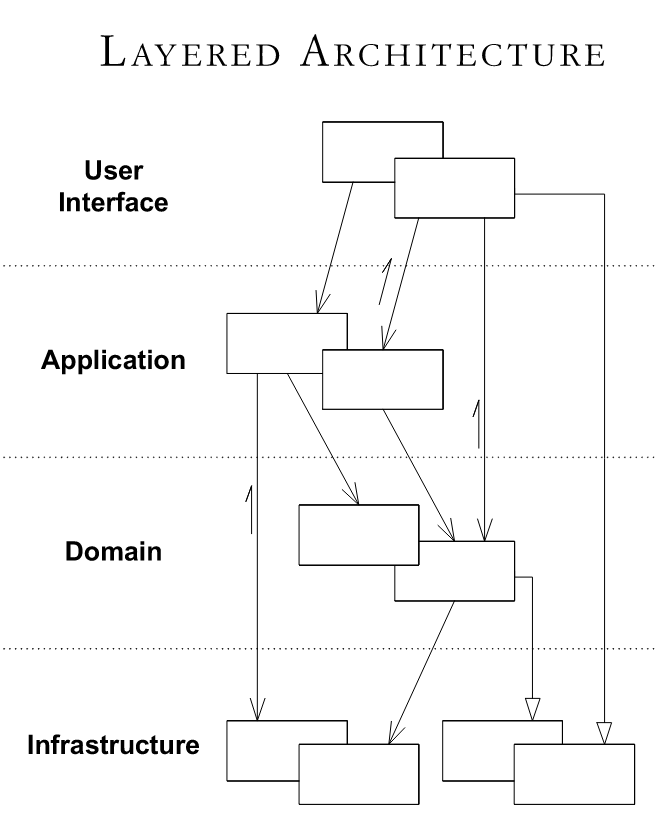
\includegraphics[scale=0.5]{domain-driven-design-layers.png}}
\end{figure}

\begin{figure}[ht]
    \caption{Graph der Modulabhängigkeiten}
    \label{module-dependency-graph}
    \centering\fbox{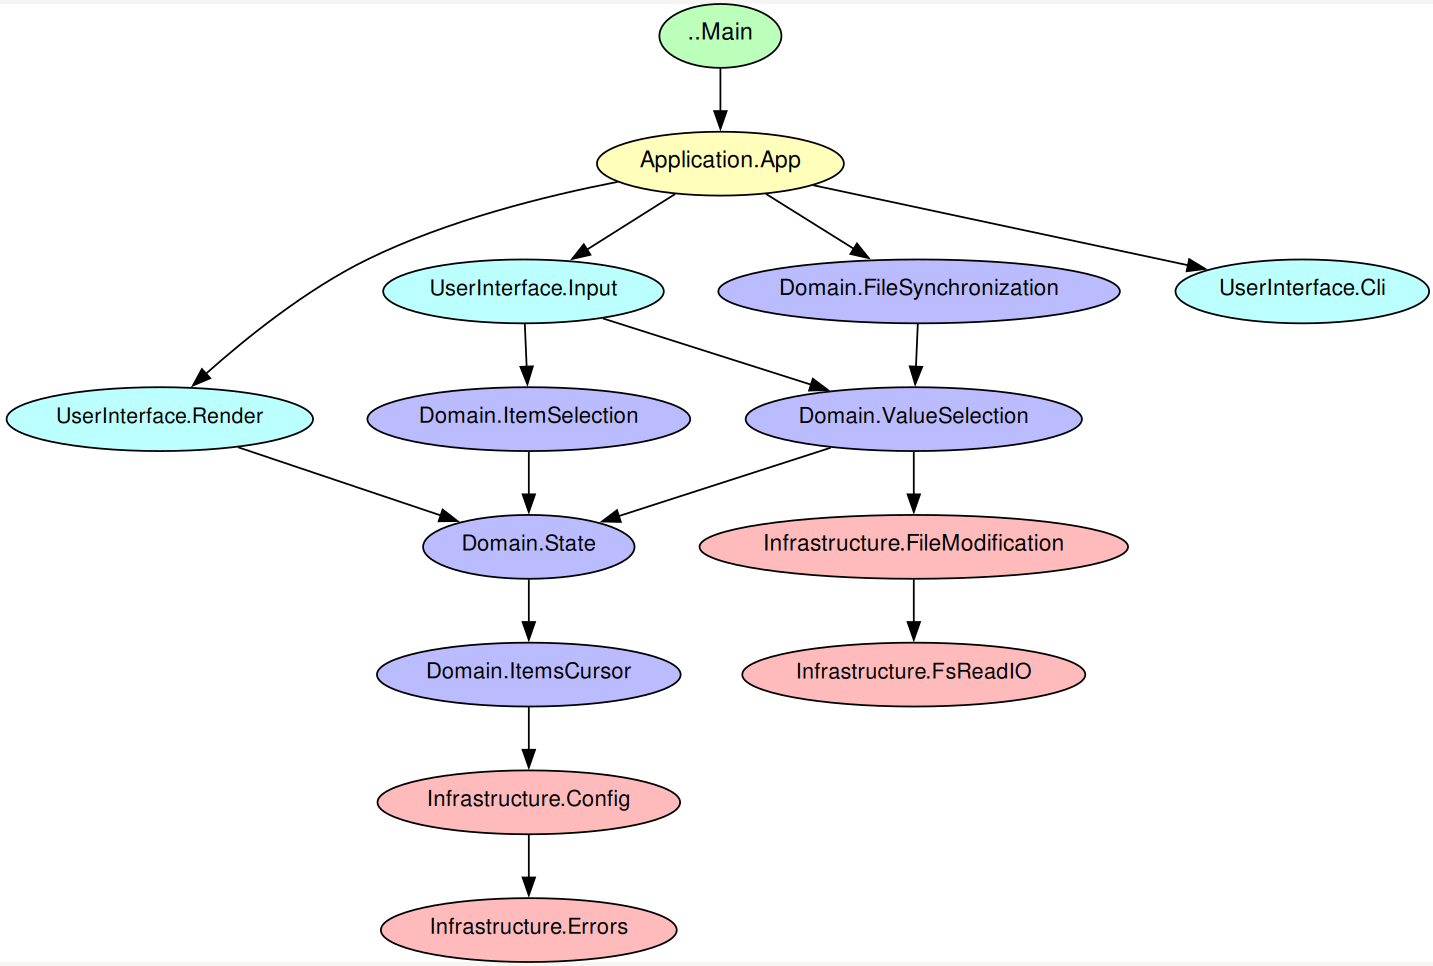
\includegraphics[scale=0.3]{module-dependency-graph.png}}
\end{figure}

\begin{figure}[ht]
    \caption{Ausgabe bei Ausführung der Testsuite}
    \label{test-suite}
    \centering\fbox{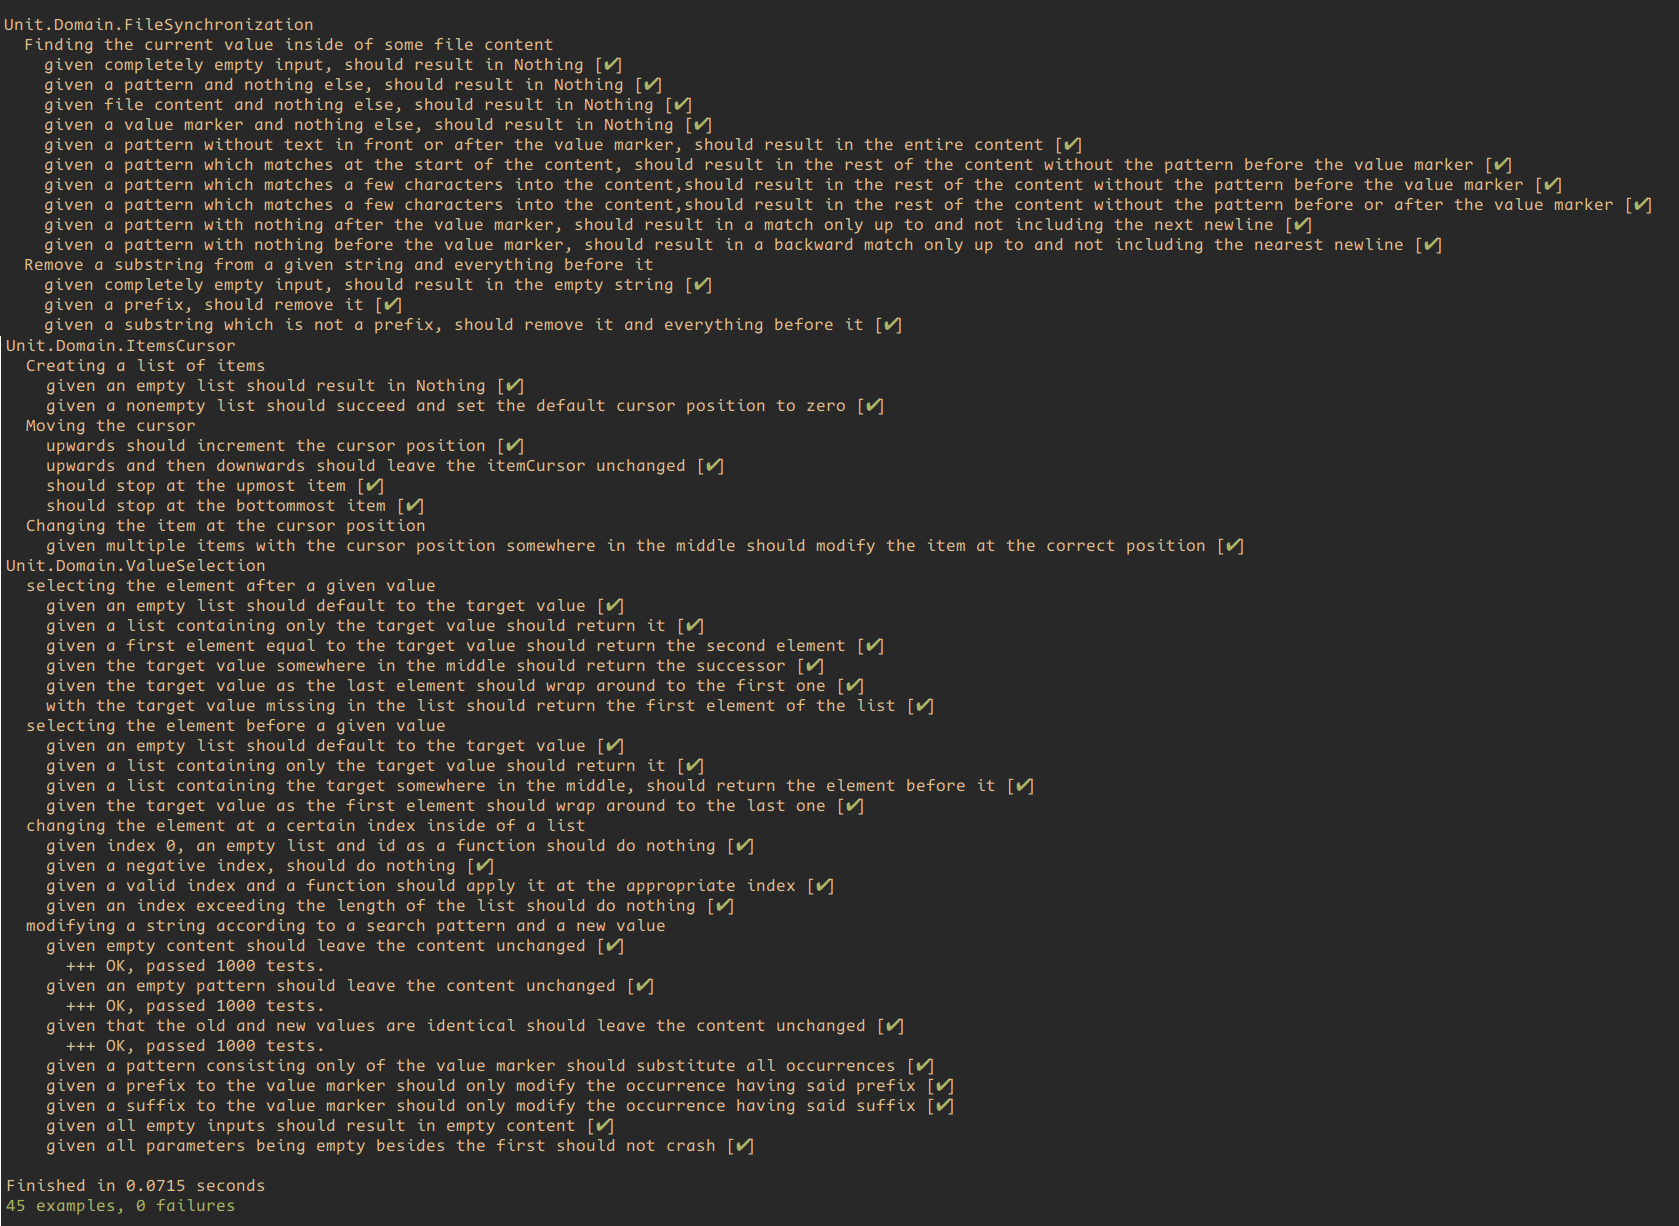
\includegraphics[scale=0.25]{full-test-suite.png}}
\end{figure}

\section{Kundendokumentation} \label{Kundendokumentation}

\subsection{Beschreibung}
Terminal-Config-Manager ist ein Linux-Programm mit welchem
\gls{Textpassage}n innerhalb meherer Dateien schnell zwischen einer Reihe
vorkonfigurierter \gls{Textpassage}n umgeschalten werden können.

Der Hauptanwendungsfall ist die effiziente  Manipulation von
Konfigurationsdateien von Softwareanwendungen, die häufig angepasst
werden müssen.

\subsection{Installation} \label{Installation}
Es wurden vorkonfigurierte Pakete für sowohl ArchLinux\cite{arch}-basierte als auch
Debian\cite{debian}-basierte Betriebssysteme bereitgestellt. Alternativ
kann das Programm auch manuell installiert werden.

\begin{center}
	\textbf{Arch-Linux \cite{arch}, via PKGBUILD Datei und pacman \cite{pacman}}
\end{center}

Im Projektverzeichnis unter

\begin{minted}[bgcolor=codebg]{bash}
	/distribution/arch/PKGBUILD
\end{minted}

befindet sich eine Spezifikationsdatei anhand derer das Softwarepaket
erstellt und anschließend installiert werden kann:

\begin{minted}[bgcolor=codebg]{bash}
	cd distribution/arch
	makepkg
	pacman -U terminal-config-manager-1.0.0-1-x86_64.pkg.tar.zst
\end{minted}

Die Deinstallation erfolgt mittels

\begin{minted}[bgcolor=codebg]{bash}
	pacman -R terminal-config-manager
\end{minted}

\begin{center}
	\textbf{Debian, via .deb Datei und dpkg\cite{dpkg}  bzw. apt\cite{apt}}
\end{center}

Im Projektverzeichnis unter

\begin{minted}[bgcolor=codebg]{bash}
	/distribution/debian/terminal-config-manager.deb
\end{minted}

befindet sich ein Softwarepaket, das mittels \mintinline{bash}{dpkg}
oder \mintinline{bash}{apt} direkt installiert werden kann.

\begin{minted}[bgcolor=codebg]{bash}
	cd distribution/debian
	dpkg --install ./terminal-config-manager.deb
	# apt install ./terminal-config-manager.deb
\end{minted}

Die Deinstallation erfolgt mittels

\begin{minted}[bgcolor=codebg]{bash}
	dpkg --remove terminal-config-manager
	# apt remove terminal-config-manager
\end{minted}

\begin{center}
	\textbf{Alternative, ohne Paketmanager}
\end{center}

Wenn das Programm nicht vom systemeigenen Paketmanager verwaltet werden
soll, dann kann es manuell kompiliert und in einem passenden
Verzeichnis abgelegt werden.

Voraussetzung hierfür ist, dass das Programm \mintinline{bash}{stack} auf dem
System installiert ist.

Im Projektverzeichnis wird mit

\begin{minted}[bgcolor=codebg]{bash}
	stack build --test --copy-bins
\end{minted}

das Programm kompiliert, die Testsuite ausgeführt und die ausführbare Datei im
Projektverzeichnis unter

\begin{minted}[bgcolor=codebg]{bash}
	bin/terminal-config-manager
\end{minted}

abgelegt. Anschließend kann das Programm in ein Verzeichnis kopiert werden, das in die
Systempfadliste eingetragen ist, beispielsweise

\begin{minted}[bgcolor=codebg]{bash}
	cp bin/terminal-config-manager ~/.local/bin
\end{minted}

Die Deinstallation erfolgt mittels

\begin{minted}[bgcolor=codebg]{bash}
	rm ~/.local/bin/terminal-config-manager
	rm <Konfigurationsdateipfad>
\end{minted}

\subsection{Konfiguration}
Die Zieldateien und -textpassagen müssen vor Ausführung des Programms
über eine Datei im YAML-Format konfiguriert werden.

\paragraph{Verzeichnis}
Das Programm erwartet, dass sich eine solche Datei in einem der folgenden
Verzeichnisse befindet. Die Reihenfolge entspricht der absteigenden Priorität
beim Vorhandensein mehrerer Konfigurationsdateien:

\begin{enumerate}
  \item ./config.yaml
  \item \$\{HOME\}/.config/terminal-config-manager/config.yaml \textbf{(empfohlen)}
  \item \$\{HOME\}/.terminal-config-manager.yaml
\end{enumerate}

Der Dateipfad 1 bezeichnet den Ort der ausführbaren Datei selbst und sollte nur
zu Debugging- oder Entwicklungszecken genutzt werden. Die Pfade 2 und 3 sind
gängige Ablageorte für nutzerspezifische Konfigurationsdateien unter Linux.

\newenvironment{code}{\captionsetup{type=listing}}{}
\SetupFloatingEnvironment{listing}{name=Abbildung}

\begin{figure}
  \caption{Beispielaufbau der Konfigurationsdatei}
  \label{fig:sample-config}
  \begin{minted}[bgcolor=codebg]{yaml}
    config_lines_to_manage:
      - title: Beispieltitel 1
        path: /home/alice/zieldatei.conf
        pattern: "'statspush_enabled' => {{value}},"
        targetValue: "true"
        possibleValues:
          - "true"
          - "false"

      - title: Beispieltitel 2
        path: /home/alice/verzeichnis/weitere-zieldatei.txt
        pattern: "SOFTWARE_ENV={{value}}"
        targetValue: production
        possibleValues:
          - testing
          - staging
          - production
          - local

      - ...
  \end{minted}
\end{figure}

\paragraph{Aufbau}
In Abb. \ref{fig:sample-config} ist der Aufbau der Konfigurationsdatei
illustriert. In \cite{latex2e}

\subsection{Benutzung} \label{Benutzung}
\paragraph{Start}
Das Programm wird nach erfolgreicher Installation mit dem Befehl

\begin{minted}[bgcolor=codebg]{bash}
    terminal-config-manager
\end{minted}

von der Kommandozeile aus gestartet. Für jeden Eintrag in der Konfigurationsdatei
zeigt das Programm eine Zeile an.

\begin{figure}
    \caption{Ansicht nach Programmstart}
    \label{post-start}
    \begin{center}
        \fbox{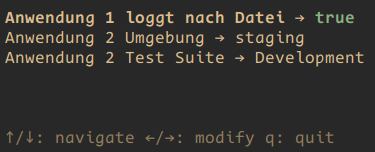
\includegraphics[scale=0.5]{post-start.png}}
    \end{center}
\end{figure}

\paragraph{Ansicht}
Abb. \ref{post-start} zeigt eine typische Ansicht direkt nach dem Start des
Programms. Die ersten drei Zeilen repräsentieren jeweils einen Eintrag in
der Konfigurationsdatei und somit eine Ziel-\gls{Textpassage} mit ihrem
aktuellen Wert. Jede dieser Zeilen besteht aus dem in der Konfigurationsdatei
vergebenen Titel des Eintrags, einem Pfeil und dem aktuellen Wert der Ziel-\gls{Textpassage}.
Die \textbf{aktuell ausgewählte Zeile} ist fett gedruckt während
\textcolor{teal}{der aktuelle Wert} der ausgewählten Zeile blau dargestellt wird.
Die genaue Darstellung ist dabei vom verwendeten Terminal-Emulator und dessen
Einstellungen bezüglich Schriftart und Farbwerten abhängig.

\paragraph{}
Die ausgegraute Zeile am unteren Rand beschreibt in Kurzform die verfügbaren
Kommandos und die davon ausgelösten Aktionen.

\paragraph{Aktionen}
Die Hauptfunktionen werden über die vier Pfeiltasten gesteuert. Die Pfeiltasten
hoch bzw. runter bewegen die Zeilenmarkierung nach oben bzw. unten. Die Pfeiltasten
links bzw. rechts schalten den zur markierten Zeile gehörigen Wert weiter zum
nächsten Wert aus der konfigurierten Liste der möglichen Werte
(siehe Kapitel \ref{Konfiguration} - Konfiguration). Beim Umschalten eines Werts
wird die zugehörige Zieldatei entsprechend modifiziert.

\paragraph{} Mit einem Tastendruck auf q kann das Programm jederzeit beendet werden
und zur Kommandozeile zurückgekehrt werden.

\subsection{Problembehandlung} \label{Problembehandlung}
\paragraph{Fehlende Konfigurationsdatei} Wenn beim Programmstart der Fehler
\begin{minted}[bgcolor=codebg]{bash}
    Error: No config file found at any of the search paths: ...
\end{minted}
auftritt, dann bedeutet das, dass bei der Suche nach Konfigurationsdateien an
keinem der angegebenen Pfade eine Datei gefunden wurde.
\paragraph{Lösung}
Es wird wie in Kapitel \ref{Konfiguration} (Konfiguration) beschrieben eine
Konfigurationsdatei an einem der validen Dateipfade angelegt. Im Dateisystempfad
unter

\begin{minted}[bgcolor=codebg]{bash}
    /usr/share/terminal-config-manager/config.yaml
\end{minted}

befindet sich eine Beispielkonfigurationsdatei, welche als Vorlage genutzt
werden kann:

\begin{minted}[bgcolor=codebg]{bash}
    mkdir ~/.config/terminal-config-manager
    cp  /usr/share/terminal-config-manager/config.yaml \
        ~/.config/terminal-config-manager
\end{minted}

\paragraph{Falsches Konfigurationsdateiformat} \label{missing-config} Wenn beim
Programmstart ein Fehler ähnlich

\begin{minted}[bgcolor=codebg]{text}
    An error occured while parsing the configuration file.
    The details are: ...
\end{minted}

auftritt, dann bedeutet das, dass die erste vom Programm gefundene Konfigurationsdatei
entweder nicht dem YAML-Format \cite{yaml} entspricht und/oder fehlende Elemente aufweist.

\paragraph{Lösung}
Die Fehlermeldung wird weitere Detailinformationen enthalten wie beispielsweise:

\begin{minted}[bgcolor=codebg]{text}
    The top level of the config file
    should be an object named 'config_lines_to_manage'
\end{minted}

anhand derer sich das Problem identifizieren lässt. Im Zweifelsfall muss dem
Kapitel \ref{Konfiguration} (Konfiguration) bzw. der Problembehandlung für
fehlende Konfigurationsdateien in Kapitel \ref{missing-config} folgend eine valide Konfigurationsdatei
per Hand angelegt werden.

\paragraph{Fehlende Dateizugriffsrechte} Wenn bei der Auswahl eines neuen Werts
der Fehler

\begin{minted}[bgcolor=codebg]{text}
    terminal-config-manager: <Zieldateipfad>: withFile:
    permission denied
\end{minted}

auftritt, dann bedeutet das, dass dem aktuellen Linux-Nutzer die nötigen
Zugriffsrechte fehlen, um die Zieldatei zu modifizieren.

\paragraph{Lösung}
Es muss sichergestellt werden, dass alle in der Konfigurationsdatei definierten
Zieldateien vom aktuellen Nutzer modifiziert werden können. Im häufigsten Fall
ist der aktuelle Nutzer nicht als \mintinline{bash}{owner} der Datei eingetragen:

\begin{itemize}
    \item Wenn dies angebracht ist, dann kann der Nutzer der Datei geändert werden:
          \begin{minted}[bgcolor=codebg]{text}
            chown <Nutzer> <Zieldateipfad>
        \end{minted}
    \item Wenn dies angebracht ist, dann können die Schreibrechte der Zieldatei
          angepasst werden:
          \begin{minted}[bgcolor=codebg]{text}
            chmod o+w <Zieldateipfad>
        \end{minted}
\end{itemize}

\textbf{Wenn keine der beiden oben genannten Optionen anwendbar ist, dann ist diese
    Zieldatei nicht für die Modifizierung durch das Programm geeignet}.

\printbibliography

\printglossaries

\end{document}